% !TeX root = ../../thesis.tex
\chapter{This is results}\label{ch:results}

\section{Zika ancestral reconstruction}

\section{Hepatitis B phylogeography}

\subsection{Temporal signal}

\subsection{Demographic reconstruction}

\subsection{Results that worked}

\subsubsection{Convergence}

\subsubsection{Tree topology}

\subsubsection{Migration history}

\ref{fig:HBV-A_phylogeo}
\ref{fig:HBV-D_phylogeo}
\ref{fig:bayes_factors}

\begin{figure}[ht]
  \centering
  \medskip
  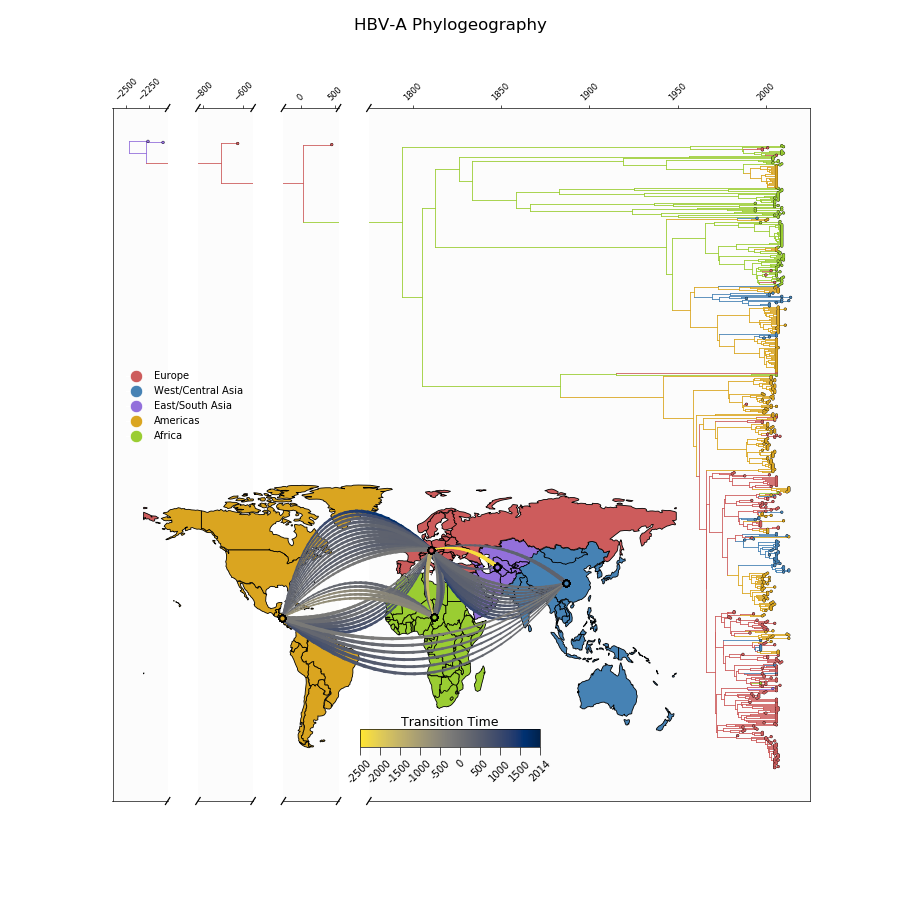
\includegraphics[width=.9\textwidth]{HBV-A_phylogeography_and_mcc_tree_smallboi}
  \caption[HBV-A phylogeography ]{Time-scalled maximum clade credibility tree representing the evolutionary history of HBV subtype A, averaged over 1,000 MCMC posterior state samples. The root is inferred to be at 2504BCE. Tip and branch colors represent location, both known and inferred by CTMC. Breaks in time axis represent long periods of time covered by individual branches. (inset) World map colored according to regions used for CTMC analysis. Each counterclockwise arrow represents an inferred transmission event between two regions (55 total). Arrow colors denote timing intervals of each introduction. Europe shows the greatest number of outgoing introductions (29). West/Central Asia is the inferred root location of the tree, with one ancient transmission to Europe inferred to have taken place between 2243--876BCE.}
  \label{fig:HBV-A_phylogeo}
\end{figure}

\begin{figure}[ht]
  \centering
  \medskip
  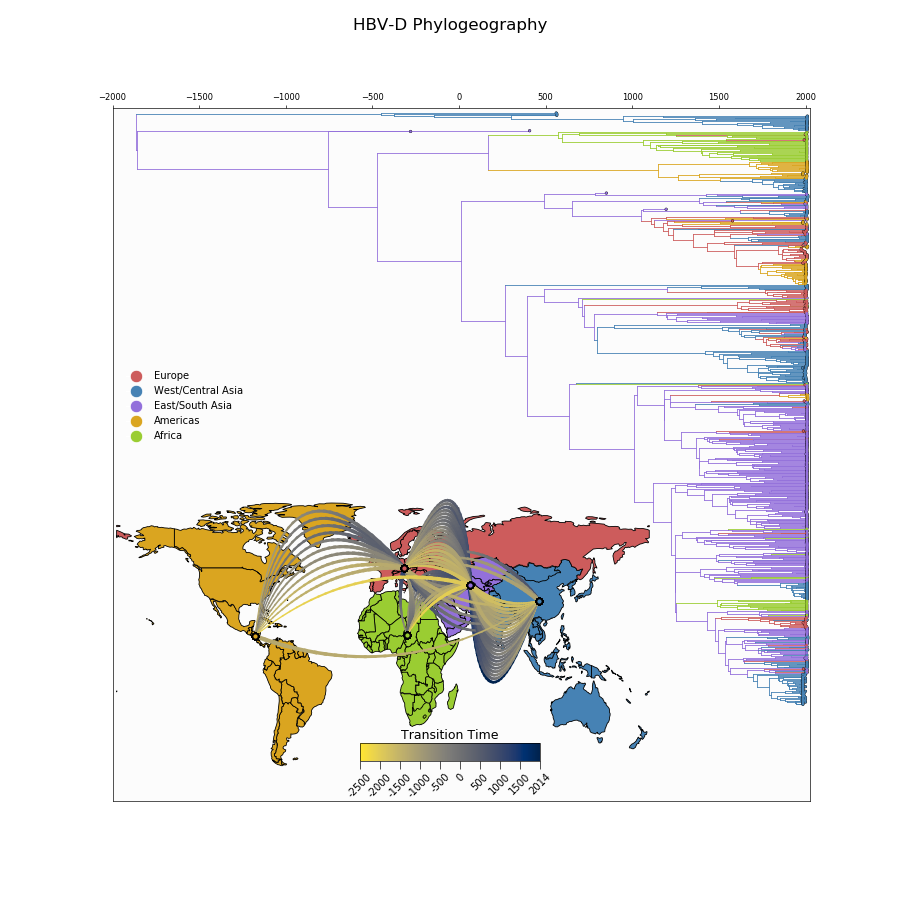
\includegraphics[width=.9\textwidth]{HBV-D_phylogeography_and_mcc_tree_smallboi}
  \caption[HBV-D Phylogeography]{Time-scaled maximum clade credibility tree representing the evolutionary history of HBV subtype D, averaged over 1,000 MCMC posterior state samples. The root is inferred to be at 1779 BCE. Tip and branch colors represent location, both known and inferred by CTMC. (inset) World map colored according to regions used for CTMC analysis. Each counterclockwise arrow represents an inferred transmission event between two regions (82 total). Arrow colors denote timing intervals of each introduction. West/Central Asia shows the greatest number of outgoing transmission events (55), as well as being the most likely location of the most recent common ancestor to sampled modern sequences.}
  \label{fig:HBV-D_phylogeo}
\end{figure}

\begin{figure}[ht]
  \centering
  \medskip
  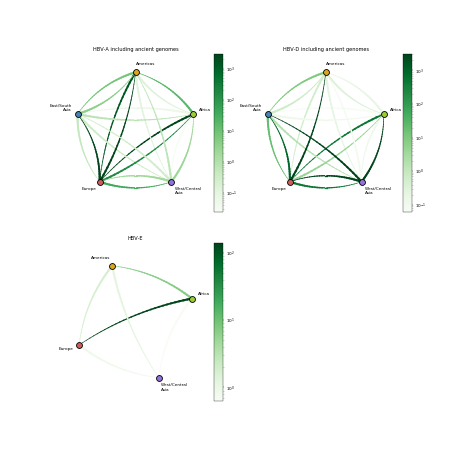
\includegraphics[width=.9\textwidth]{bayes_factors_smallboi}
  \caption[Bayes' factors of HBV geographic transitions]{Networks summarizing posterior support for migrations between geographic regions as determined by BSSVS analysis. Inferred migrations are represented as counterclockwise arrows. Bayes' factors are represented by color intensity; darker arrows depict higher Bayes' factors, therefore higher posterior support. In HBV-A we observe well supported inference of migrations out of Europe to all other regions, as well as high support for inferred migrations into Europe from Africa and the Americas. In HBV-D we observe well supported migration history from Africa to Europe, and from Europe to the Americas and Asia. Finally, in HBV-E we observe very well supported migration inference from Africa to Europe, as well as relatively high support for migration from Africa to the Americas.}
  \label{fig:bayes_factors}
\end{figure}

\section{Lassa phylogenetics}





%%%%%%%%%%%%%%%%%%%%%%%%%%%%%%%%%%%%%%%%%%%%%%%%%%
% Keep the following \cleardoublepage at the end of this file,
% otherwise \includeonly includes empty pages.
\cleardoublepage

% vim: tw=70 nocindent expandtab foldmethod=marker foldmarker={{{}{,}{}}}
